\subsubsection{Spreminjanje lastnosti}

V tem odseku bom opisal zapis spreminjanja lastnosti,
katerega lahko uporabimo v generičnem modelu, v primerih
ko želimo uporabiti storitev, ki nima lastnosti,
katere storitev zahteva.

Denimo da zahteva 2 2 iz slike~\ref{fig:generic-services},
zahteva lastnost \textit{Nestrukturirani podatki (NS)},
ki je \textit{storitev 3} ne podpira,
saj podpira \textit{Strukturirane podatke (S)}.
Med \textit{zahtevo 2 2} in \textit{storitev 3}
vmestimo \textit{storitev 4},
ki opravi transformacijo.
Nov model je prikazan v sliki~\ref{fig:transform}.

\begin{figure}[H]
    \centering
    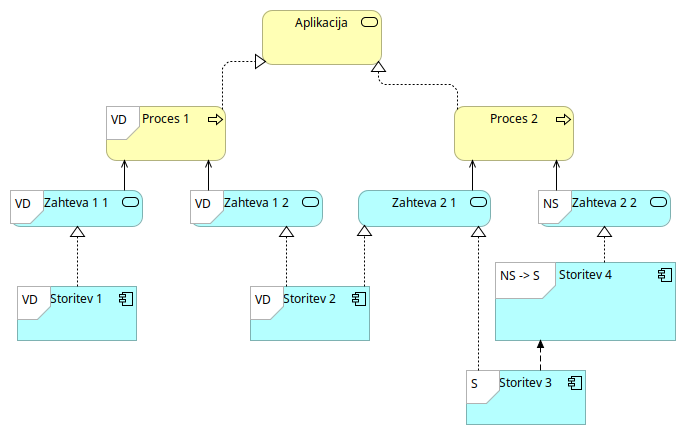
\includegraphics[width=0.9\textwidth]{img/gradnja/generic-transformation.png}
    \caption{Transformacija lastnosti v modelu.}
    \label{fig:transform}
\end{figure}
